\section{Performance Evaluation}~\label{sec:experiments}
%In this section, we present

In this section, we present microbenchmarck experiments to measure the efficiency of the scheme and macrobenchmark experiments to demonstrate its performance in large-scale database.

\subsection{Experiment Setup}
In order to demonstrate the feasibility of \name, we implement it by using Crypto++ 5.6.5. The prototype is written by about 2200 lines of code. %Our implementation includes all the algorithms mentioned in section \uppercase\expandafter{\romannumeral4}.
We implement two random-oracles with HMAC-SHA256 and use 128-bit AES-CBC to encrypt the authenticators. The hash function is an implementation of SHA3-256 and the incremental hash function is MuHash.

Our experiments were performed by using a machine with single thread on an Intel Core i5 2.5GHz processor with 4G RAM. %All experiments w performed
We used the Enron email dataset~\cite{enron_email} in our experiments. The used part of the dataset~\cite{enron_email} is between ``allen-p" and ``kaminski-v". We extract document-keyword pairs from the dataset and construct our plain-text inverted index by using a python script. Note that the delays of extracting keywords from files are not included in our evaluation, since keyword extraction is independent with \name. We use microbenchmark experiments to measure the overheads of the algorithms proposed. Here, we measure the average results with ten runs of experiments. In macro-benchmark experiments, we evaluate the \name performance in large-scale database by feeding the measured delays and then we compare \name with the existing SSE scheme~\cite{cash2014dynamic}.
%Each data point in the graphs is an average of ten trials.
%The part of the Enron email dataset that we used in our experiments is between "allen-p" and "kaminski-v".
\subsection{Microbenchmark}


\begin{figure*}[bhpt]
\centering
  \begin{minipage}[b]{0.33 \textwidth}
    \includegraphics[width=\textwidth]{initialization}
    \caption{$Init$ delays}
    \label{fig:initialization}
  \end{minipage}
  \hspace{-0.2in}
  \begin{minipage}[b]{0.33 \textwidth}
    \includegraphics[width=\textwidth]{update}
    \caption{$Update$ throughput}
    \label{fig:update}
  \end{minipage}
  \hspace{-0.25in}
  \begin{minipage}[b]{0.33 \textwidth}
    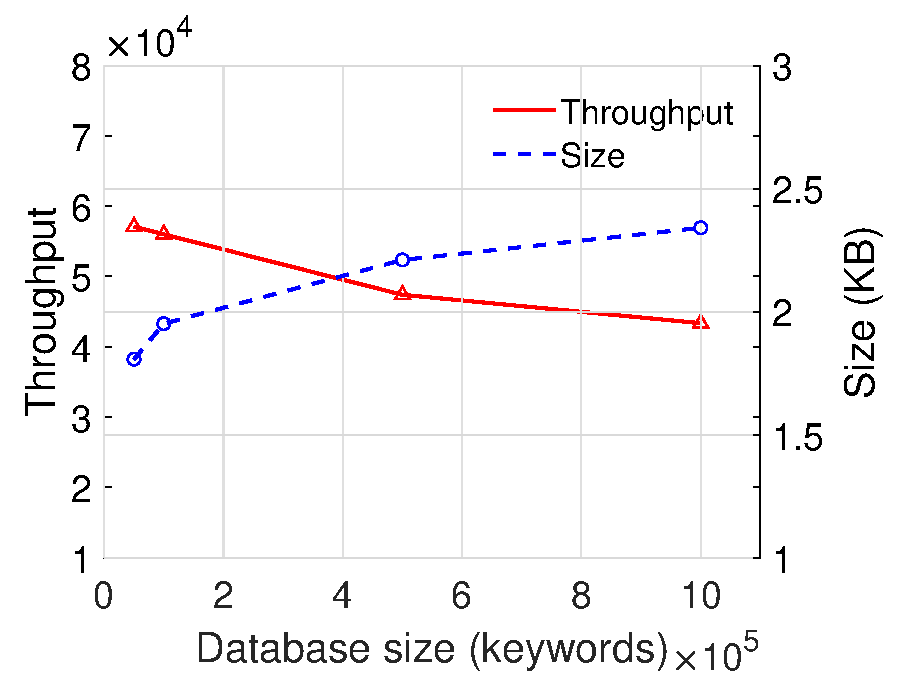
\includegraphics[width=\textwidth]{prove}
    \caption{$Prove$ cost}
    \label{fig:prove}
  \end{minipage}

  \hspace{-40.0pt}
  \par \vspace{-10.pt}
  \hspace{-36.0pt}

  \begin{minipage}[b]{0.33 \textwidth}
    \includegraphics[width=\textwidth]{proof}
    \caption{Proof cost}
    \label{fig:proof}
  \end{minipage}
  \hspace{-0.2in}
  \begin{minipage}[b]{0.33 \textwidth}
    \includegraphics[width=\textwidth]{generate}
    \caption{$Generate$ performance}
    \label{fig:generate}
  \end{minipage}
  \hspace{-0.2in}
  \begin{minipage}[b]{0.33 \textwidth}
    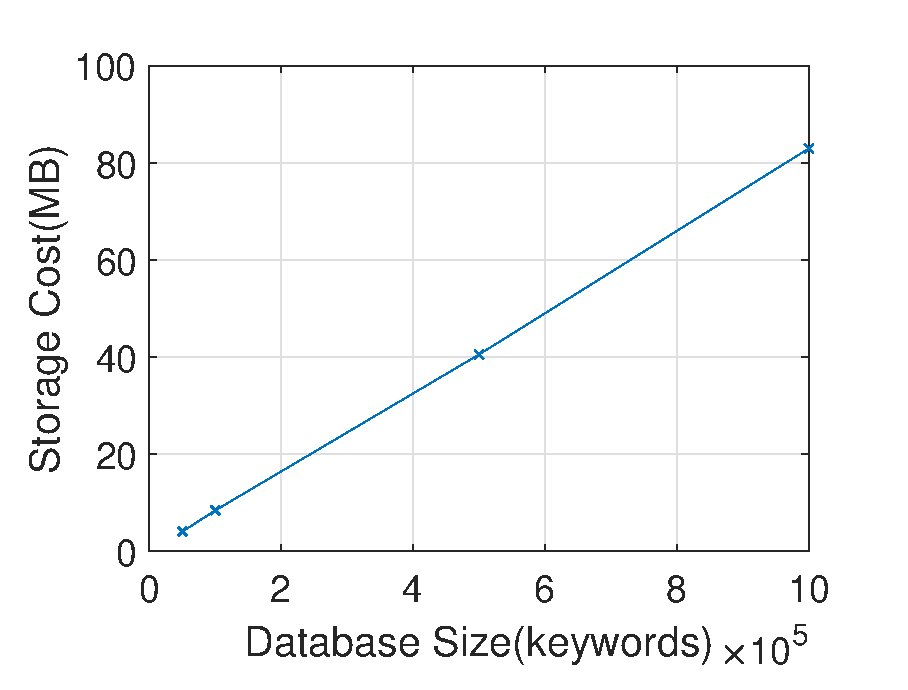
\includegraphics[width=\textwidth]{storage}
    \caption{Storage cost of MPT}
    \label{fig:storage}
  \end{minipage}

  \hspace{-40.0pt}
  \par \vspace{-10.pt}
  \hspace{-36.0pt}

  \begin{minipage}[b]{0.33 \textwidth}
    \includegraphics[width=\textwidth]{verify}
    \caption{$Verify$ latency}
    \label{fig:verify}
  \end{minipage}
  \hspace{-0.2in}
  \begin{minipage}[b]{0.33 \textwidth}
    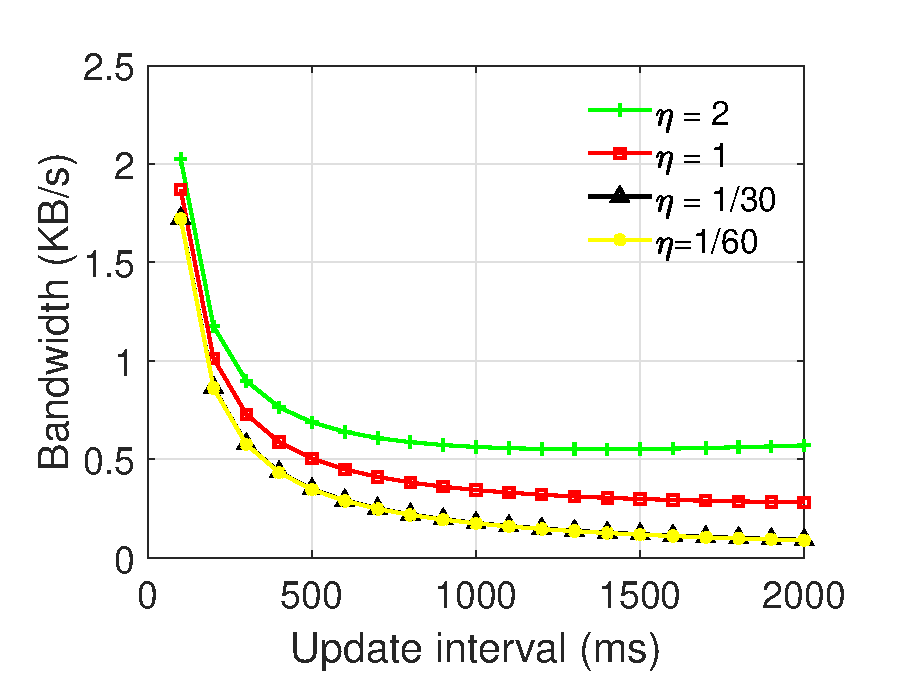
\includegraphics[width=\textwidth]{bandwidth}
    \caption{Bandwidth consumption}
    \label{fig:authenticator bandwidth}
  \end{minipage}
  \hspace{-0.2in}
  \begin{minipage}[b]{0.33 \textwidth}
    \includegraphics[width=\textwidth]{comparison}
    \caption{\blue{Comparison with SSE~\cite{cash2014dynamic}}}
    \label{fig:comparison}
  \end{minipage}
\centering
\end{figure*}


First, we measure the initialization delays in building the proof index. As shown in Fig.~\ref{fig:initialization}, the delays of generating the proof index are proportional to the size of the document-keyword pairs, since \name performs the same number of insertions to the number of the document-keyword pairs. Overall, the initialization consumes around 25 seconds where the documents include four million keywords, which is acceptable.
% for the initialization process.

The update delays are decided by the size of the database that is measured by the number of keywords. The size of MPT grows with the increase in the number of keywords. Strictly speaking, the delays are directly related to the number of the layers in MTP. In order to show the relationship between the update delays and the database size, we use various numbers of keywords to measure the delays. Since the number of keywords varies from each file, we use throughput to measure the number of keyword-document pairs that can be updated per second (see Fig.~\ref{fig:update}). We observe that the throughput of adding and deletion operations are almost the same. The throughput decreases when the size of the database grows. They can support 110,000 updates per second with one million keywords database.
Similarly, we observe that the bandwidth overhead incurred by update token is decided by the number of keywords contained in the file, which is acceptable as well.

%\subsection{Microbenchmark: {\it Prove} and {\it Rebuild}}
%We use throughput to measure our prove algorithm. Prove process is actually the process of searching and tracing back in the proof index. As a result, the performance
As shown in Fig.~\ref{fig:prove}, the server can perform about 43,000 prove operations per second even when the size of the database is one million keywords, which indicates the server can simultaneously support 43,000 concurrent queries submitted by users.
%the throughput of {\it Prove} is better that the {\it Update} algorithm.
The communication overhead incurred by proof delivery is only a few kilobytes, which is decided by the number of layers in MPT, and gradually increases as the database grows (see Fig.~\ref{fig:proof}). Also, we measure the performance of {\it Generate} operations performed by the data users.
% and usually is not frequent operations.  %Hence, we only measure the delays of rebuilding operations. % rather than the throughput. We prove through experiments that
We observe that the delays of generating root are within 0.1 milliseconds (see Fig.~\ref{fig:generate}) and are acceptable. The storage overhead of our proof index is shown in Fig.~\ref{fig:storage}. If we use a database with 1,000,000 keywords, the storage overhead is about 82MB. Compared with the size of the original dataset itself,i.e., 590MB, the overhead is relatively small. Note that, if a data owner stores various media types of data set (e.g., images or music) with fewer keywords or attributes, the storage overhead of MPT is negligible compared with the size of the data set itself.

%For a 590MB database with 1,000,000 keywords, the storage cost of the MPT is only about 82MB. As the data set (aka, the Enron email) contains a large number of keywords, the storage space of MPT is relatively large. Note that, if a data user stores various media types of data set (e.g., images or music) with fewer keywords or attributes, the storage overhead of MPT is negligible compared with the size of the data set itself.


\subsection{Macrobenchmark}
%The cost of preventing the replay attack consists of the following two parts: the computational cost of the data user for executing the verify algorithm and the communication cost of the data owner for updating the authenticator. Here we evaluate the cost of preventing the replay attacks from these two aspects.
In this experiment, we measure the delays of verification and the communication overhead in data owners. %Here, we assume that, for a data owner, the data update frequency is constant.  %represented by $\eta$ is constant, and the update interval is represented by $\alpha$.
Firstly we evaluate the verification delays in data users (see Fig.~\ref{fig:verify}). Here, $\eta$ is the update frequency of the data owner, we assume the time that a user initiates a query is uniformly distributed during an update interval, and then the user's waiting delays are also uniformly distributed. Therefore, the expected delay is half of the update interval, and the verification delays are dominated by the waiting delays. Note that an entire verification delay includes the delay of waiting for a checkpoint and the delay of executing the {\it Check} and the {\it Generate} algorithms. Since the execution delay of the {\it Generate} algorithm is relatively stable, we do not plot it in Fig.~\ref{fig:verify}. The execution delay of the {\it Check} algorithm is proportional to the update interval, which is mainly incurred by decrypting authenticators. In a later experiment, we will show that we can set an update interval so as to make a trade-off between verification delays and communication overhead.
%As we observed, the average delay for decrypting each authenticator is only about 0.12 milliseconds.
%Overall, the verification delay is around 500 milliseconds.}
%is negligible compared with the waiting delays,
%We observe that the verification delays are dominated by the waiting delays.
%delays of performing the {\it Check} algorithm. We observe that the execution delay of the {\it Check} algorithm is proportional to the number of rounds that are required to trace back in the timestamp chain. %As the worst case, the delay is  to the number of rounds of tracing back.
%If the data update frequency is constant for a specific data owner, then the execution delays will be proportional to the update interval.}
%We denote the average decryption time of an authenticator as $avg(Dec_K(\pi))$. Then the execution time of the check algorithm can be evaluated by the following formula: $$time = \eta \times \alpha \times avg(Dec_K(\pi))$$
%Overall, the average delay of is about 0.12 milliseconds.
%, so we set $avg(Dec_K(\pi)=0.12)$.
%As shown in Figure~\ref{verify}, the execution delays of {\it Verify} mainly are decided by the waiting time, e.g., the length of the update intervals.
%Therefore, the data update frequency has small effects on the total verification delays.
%the data update frequency $\eta$
%unless it reaches several hundred times per second.
%However, In this case, the check time will take several tens of milliseconds, but the wait time is still the dominant factor.



%To evaluate the relationship between the bandwidth of the authenticator and the update interval on the data owner, we first give the formula of the bandwidth cost introduced by the authenticator as follows: $$bandwidth=\frac{\eta^2b}{2}\times \alpha + \frac{b}{\alpha}+\frac{3\eta b}{2}$$
%where $b$ is the length of the concatenation $rt||tp$. The bandwidth of the authenticator includes two part: the overhead introduced by the fixed update point and the overhead introduced by the data update.
%We present the bandwidth cost of the update frequency $\eta$ at different values as shown in

%\subsection{Communication Overheads}
Fig.~\ref{fig:authenticator bandwidth} shows the bandwidth costs for authenticator update. %Here, $b$
Here, the size of the first authenticator in each update interval is around 48 bytes, which includes 32 bytes of the root of MPT, 8 bytes of the timestamp, and an 8 bytes AES-CBC extension. Overall, the bandwidth of the authenticator includes two part: the overhead introduced by the fixed update time point and the overhead introduced by the data update. We can observe that the bandwidth cost increases to about 0.5 Kbps when the update interval decrease to zero, this is introduced by the fixed update time point which is inversely proportional to the bandwidth overhead. Moreover, the bandwidth gradually increased when the update interval becomes too long. This overhead is introduced by the length of the authenticator because as the update interval grows, the length of the authenticator becomes larger. Overall, the cost should be acceptable to achieving \name. According to the results, in order to make a decent tradeoff between verification delays and bandwidth costs, we suggest choosing an update interval between 500 milliseconds and 1,500 milliseconds.




% there is a minimum value for this curve and the bandwidth becomes large when the update interval decrease to zero, this is introduced by the fixed update interval which is inversely propotional to the bandwidth overhead. Moreover, the bandwidth gradually increased when the update interval becomes too long. This overhead is introduced by the length of the authenticator because as the update interval grows, the length of the authenticator becomes larger under the condition that the update frequency $\eta$ is a constant value.
%Consider both the latency required for the verification algorithm and the bandwidth required by the authenticator, we can appropriately choose an update interval between 500ms and 1500ms. Anyway, the selection of the update interval is a trade-off, the data owner should select approproate update interval according to his own update frequency.

\subsection{Comparison with Existing Schemes}
We combine our verifiable SSE framework, i.e., the \name scheme, with a concrete implementation of dynamic SSE scheme proposed by Cash et.al~\cite{cash2014dynamic}, and show that the additional overhead introduced by \name scheme is not large.

In order to fairly compare the schemes, we experimented with the same dataset and parameters on our machine. As shown in Fig.~\ref{fig:comparison}, we tested the overhead of the initialization phase, the search phase and the update (add and delete) phase in both schemes, in which the initialization phase is the $Init$ operation of two million document-keyword pairs and the time unit is seconds, the other three phases is the test of a single operation with a 10,000 keywords database and the time unit is microseconds. Note that the search phase in SSE corresponds to the $Prove$ operation in \name. As seen from Fig.~\ref{fig:comparison}, our \name scheme introduces very little overhead. The overhead of the $Init$ operation in our scheme only takes 1.9\% that of the entire initialization phase and is significantly smaller than the dynamic SSE scheme relatively. Moreover, for a single $Prove$ operation, our \name scheme only introduces an additional overhead of 14 microseconds for the server and only takes 2\% that of the entire search phase. And for a single $Add$ or $Delete$ operation, our \name scheme only introduces 27 microseconds overhead and takes 17\% that of the entire add or delete phase.

\blue{In Table.~\ref{tab:compareSSE}, we report the average communication overhead on the basis of 50,000 runs. The average size of search results in SSE scheme \cite{cash2014dynamic} is about 53 kb, while our proof only needs 3 kb, which means the additional overhead introduced by \name is less than 6\%. Moreover, the SSE scheme~\cite{cash2014dynamic} generates 390 bytes search tokens on average, while our search tokens are only 32 bytes, i.e., the additional overhead is less than 9\%. It shows that the overhead incurred by \name is acceptable.}

\begin{table}[h]
  \begin{center}
  \caption{Comparison with the SSE scheme proposed by Cash et al. \cite{cash2014dynamic}}
  \label{tab:compareSSE}
  %\begin{threeparttable}
  \begin{tabular}{|c|c|c|}
    \hline
    Communication cost   & SSE\cite{cash2014dynamic} &\name          \\
    \hline
    Search token          & 390 Bytes                 & 32 Bytes       \\
    \hline
    Search result/proof   & 53 Kilobytes              & 3 Kilobytes          \\
    \hline
  \end{tabular}
\end{center}
\end{table}

%We compare \name with a dynamic SSE scheme proposed by Cash et.al ~\cite{cash2014dynamic} that is mostly related to \name though it cannot provide search verifiability. % to show our DV scheme is practical.
%Both of our experiments use the Enron email dataset, in order to compare with their scheme,
%For simplicity, we directly use the experiment results in \cite{kamara2012dynamic} as baseline.
%In order to fairly compare the schemes, we set the same experimental parameters~\cite{kamara2012dynamic} in our experiments and measure the worst delays of different operations of \name. Note that, since the machine used in our experiments is much less powerful than that used in~\cite{kamara2012dynamic}, the baseline will be much worse if we repeat the experiments in~\cite{kamara2012dynamic} in our machine.
%carried on the comparison experiment as shown in \cite{comparison2} They experiment with 16MB emails and give the upperbound overhead for the search and update operations.
%For evaluating the search overhead, they give the longest search time for the keyword containing the largest number of files (about 7800 files in 16MB emails). We calculated the lower bound of their search time according to the assumption that the search time is proportional to the searched files.
%By using a 16 MB database (about 83,000 keywords), the prove operation in \name takes around 18 microseconds regardless of the number of files that contains a keyword, which is significantly efficient compared to \cite{kamara2012dynamic}.
%For evaluating the update overhead, they also give the upper bound of the Add and Delete operations, i.e., the time cost of the file containing the largest number of keywords (about 85 keywords in 16MB emails).
%For adding and deletion operations, the scheme in \cite{kamara2012dynamic} takes about 1.7 and 113 milliseconds, respectively. %We obtained through our experiment
%However, \name only takes 0.7 milliseconds to update files,
%when the database size is 16MB,
%which is significantly smaller than that in \cite{kamara2012dynamic}, especially for the delete operations.
